%%%%%%%%%%%%%%%%%%%%%%%%%%%%%%%%%%%%%%%%%
% Beamer Presentation
% LaTeX Template
% Version 1.0 (10/11/12)
%
% This template has been downloaded from:
% http://www.LaTeXTemplates.com
%
% License:
% CC BY-NC-SA 3.0 (http://creativecommons.org/licenses/by-nc-sa/3.0/)
%
%%%%%%%%%%%%%%%%%%%%%%%%%%%%%%%%%%%%%%%%%

%----------------------------------------------------------------------------------------
%	PACKAGES AND THEMES
%----------------------------------------------------------------------------------------

\documentclass{beamer}
\usefonttheme[onlymath]{serif}

\mode<presentation> {

\usetheme{Madrid}

\makeatletter
\setbeamertemplate{footline}
{
	\leavevmode%
	\hbox{%
		\begin{beamercolorbox}[wd=.333333\paperwidth,ht=2.25ex,dp=1ex,center]{author in head/foot}%
			\usebeamerfont{author in head/foot}\insertshortauthor%~~\beamer@ifempty{\insertshortinstitute}{}{(\insertshortinstitute)}
		\end{beamercolorbox}%
		\begin{beamercolorbox}[wd=.333333\paperwidth,ht=2.25ex,dp=1ex,center]{title in head/foot}%
			\usebeamerfont{title in head/foot}\insertshorttitle
		\end{beamercolorbox}%
		\begin{beamercolorbox}[wd=.333333\paperwidth,ht=2.25ex,dp=1ex,right]{date in head/foot}%
			\usebeamerfont{date in head/foot}\insertshortdate{}\hspace*{2em}
			\insertframenumber{} / \inserttotalframenumber\hspace*{2ex} 
	\end{beamercolorbox}}%
	\vskip0pt%
}
\makeatother
\setbeamertemplate{bibliography item}[text]

}

\usepackage{graphicx} % Allows including images    
\graphicspath{{../figures/}, {../figures/growthrates/}, {../figures/correlations/}, {../python/Hamiltonian/figures/}}
\usepackage{booktabs}                       
\usepackage{amsmath,amsthm,amssymb}  
\usepackage{cancel}

\usepackage[sorting=none, url=false]{biblatex}
\bibliography{../global.bib}

\renewcommand{\bf}{\mathbf}
\renewcommand{\cal}{\mathcal}
\renewcommand{\L}{\cal{L}}
\newcommand{\pd}[2]{\frac{\partial #1}{\partial #2}}
\newcommand{\pdn}[3]{\frac{\partial^{#3} #1}{\partial #2^{#3}}}
\newcommand{\pdop}[1]{\frac{\partial}{\partial #1}}
\newcommand{\nd}[2]{\frac{d #1}{d #2}}
\newcommand{\ndn}[3]{\frac{d^{#3} #1}{d #2^{#3}}}
\newcommand{\ndop}[1]{\frac{d}{d #1}}
\newcommand{\dt}{\frac{d}{dt}}
\newcommand{\grad}{\bm\nabla}
\newcommand{\cross}{\times}
\newcommand{\curl}{\grad\cross}
\newcommand{\imp}{\Longrightarrow\quad}
\newcommand{\abs}[1]{\left|#1\right|}
\newcommand{\half}{\frac{1}{2}}
\newcommand{\third}{\frac{1}{3}}
\renewcommand{\th}[1]{\frac{1}{#1}}
\renewcommand{\k}{4\pi\epsilon_0}
\newcommand{\eps}{\epsilon}
\newcommand{\intt}{\int_{t_1}^{t_2}}
\newcommand{\inti}{\int_{-\infty}^{+\infty}}
\newcommand{\ex}[1]{\left\langle #1 \right\rangle}
\newcommand{\oom}[1]{\times 10^{#1}}
\renewcommand{\d}{\delta}
\newcommand{\e}{\text{e}}
\renewcommand{\l}{\ell}
\newcommand{\om}{\omega}
\newcommand{\h}{\hbar}
\renewcommand{\t}{\tau}
\newcommand{\ket}[1]{\left|#1\right\rangle}
\newcommand{\bra}[1]{\left\langle#1\right|}
\newcommand{\braket}[2]{\left\langle#1\middle|#2\right\rangle}
\newcommand{\brakett}[3]{\left\langle#1\middle|#2\middle|#3\right\rangle}
\newcommand{\nn}{\nonumber\\}

\DeclareMathOperator{\Tr}{Tr}

%----------------------------------------------------------------------------------------
%	TITLE PAGE
%----------------------------------------------------------------------------------------

\title[Thermalization]{Thermalization in Hamiltonians\\and random unitary circuits} % The short title appears at the bottom of every slide, the full title is only on the title page

\author{Charles Stahl} % Your name

\date{\today} % Date, can be changed to a custom date

\begin{document}

\begin{frame}
\titlepage % Print the title page as the first slide
\end{frame}

\begin{frame}
\frametitle{Overview} % Table of contents slide, comment this block out to remove it
\tableofcontents % Throughout your presentation, if you choose to use \section{} and \subsection{} commands, these will automatically be printed on this slide as an overview of your presentation
\end{frame}

%----------------------------------------------------------------------------------------
%	PRESENTATION SLIDES
%----------------------------------------------------------------------------------------

\section{Introduction: thermalization}

\begin{frame}{Closed quantum systems}
In quantum mechanics we considered closed quantum systems, but then we became sophisticated and considered open quantum systems.
\begin{figure}
	\centering
	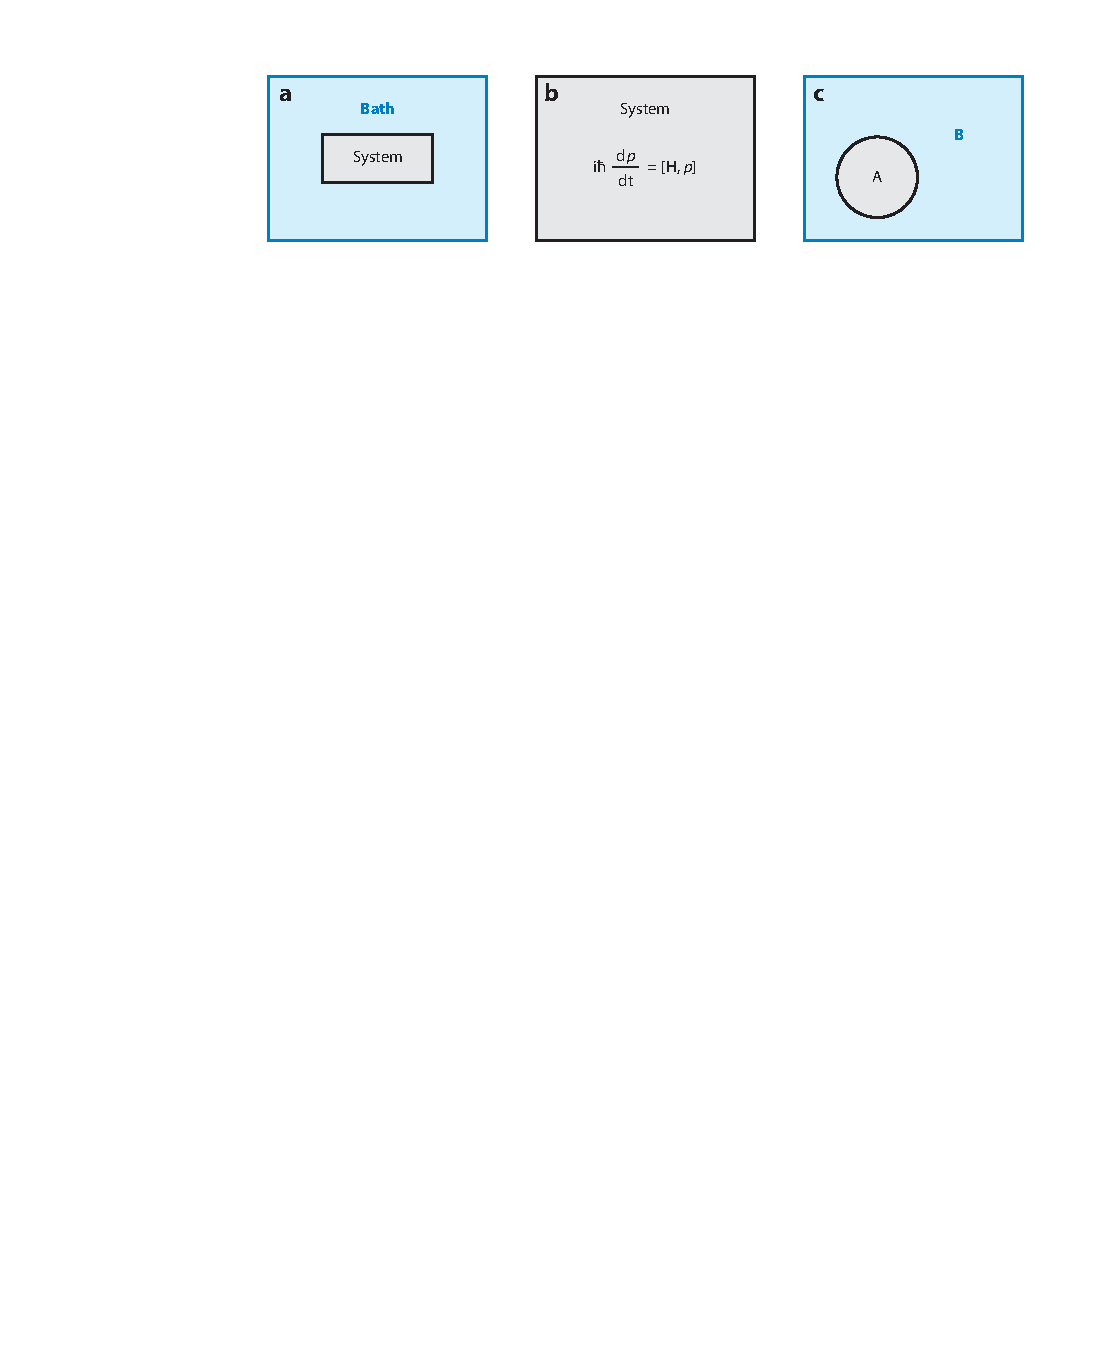
\includegraphics[width=1\linewidth]{nandkishore_huse}
	\caption{Closed and open quantum systems [Nandkishore, Huse, 2015]}
\end{figure}
Now we'll go back to studying closed quantum systems, with a twist.\\
But then how can we still have thermalization? (Subsystem looks thermal at late time)
\end{frame}

\begin{frame}{Thermalization in quantum systems}
\begin{columns}
	\begin{column}{0.7\textwidth}  %%<--- here
	Contradiction? Unitarity vs. Information Loss
	\begin{itemize}
		\item Quantum mechanics
		\item Fluid dynamics
		\item Thermodynamics
		\item Black holes
	\end{itemize}
	Resolution: Information Spreading
	\begin{itemize}
		\item Information not destroyed but spread
		\item Not accessible to local measurements
	\end{itemize}
	\end{column}
	\begin{column}{0.3\textwidth}
		\begin{figure}
			\centering
			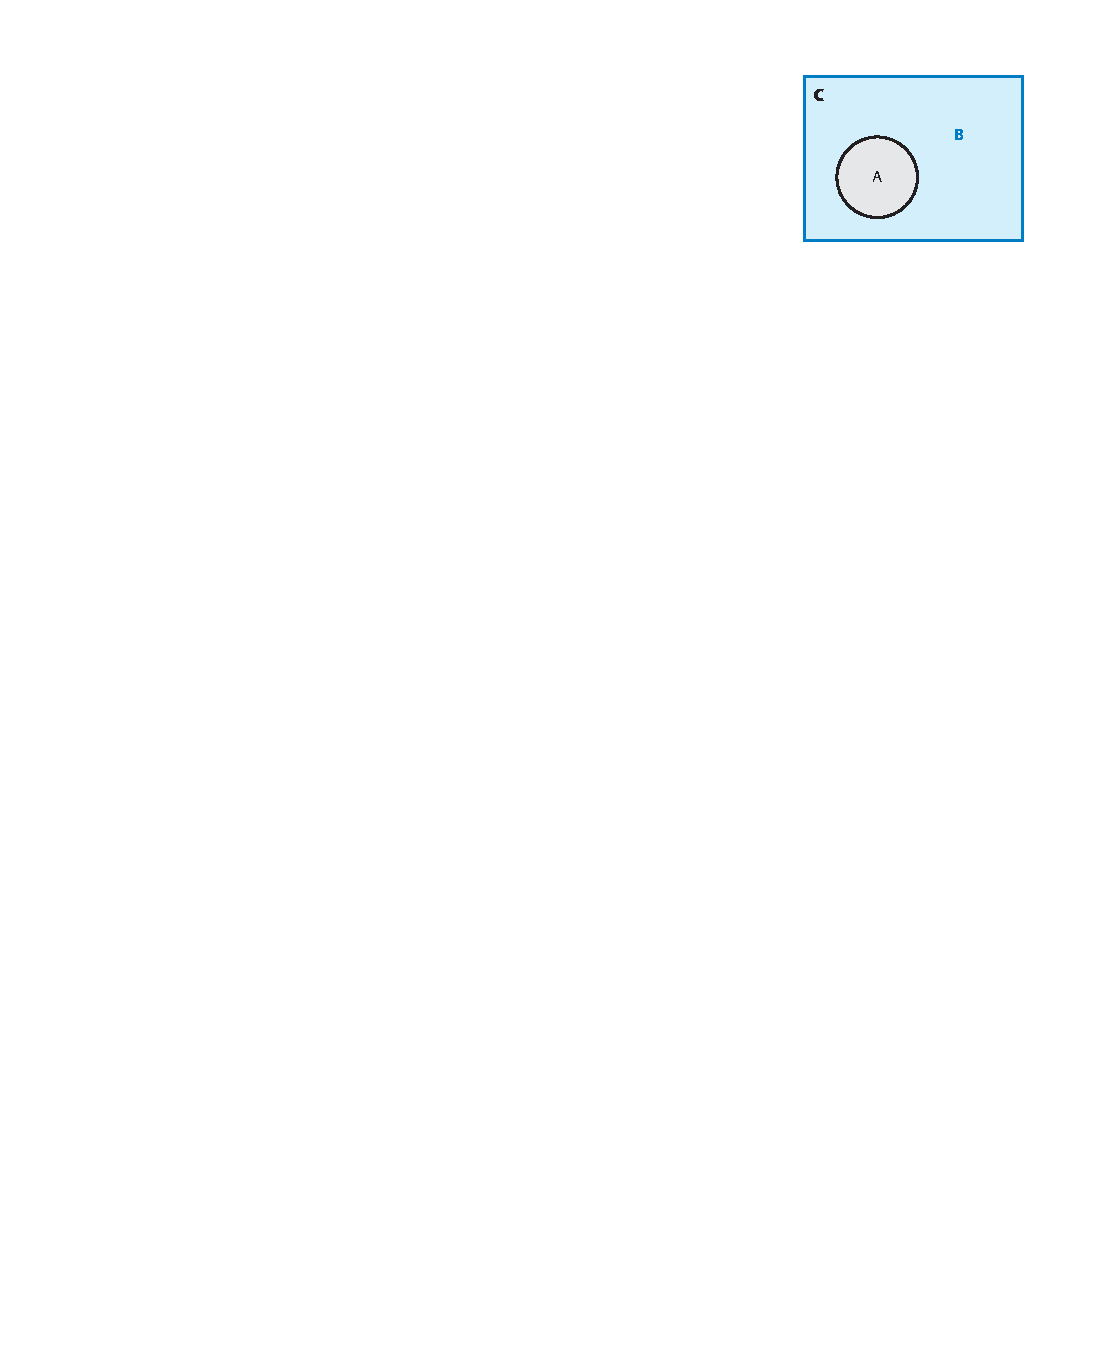
\includegraphics[width=\linewidth]{nandkishore_huse2}
		\end{figure}
	\end{column}
\end{columns}
\end{frame}

\begin{frame}{Thermalization in quantum systems}
System acts as a bath, but for what quantity?\\
\begin{itemize}
	\item In thermodynamics, any (exchanged) conserved quantities
	\item In our systems, even energy may not be conserved
	\item Entropy is conserved $\rightarrow$ exchanging entanglement
\end{itemize}
Eigenstate thermalization hypothesis.
\begin{itemize}
	\item Full-system eigenstates don't evolve
	\item But subsystem must look thermal at late time
	\item Then subsystem must look thermal at all time
	\item Applies to any system that thermalizes
\end{itemize}
\end{frame}

\section{Measures of thermalization}

\begin{frame}{Measures of thermalization}
We will look at systems with discrete space, and either discrete or continuous time.
We will be studying the spreading of operators, so we will use the Heisenberg picture,
\begin{align}
\mathcal{O}_0(t) &= e^{iHt}\mathcal{O}_0e^{-iHt}\nonumber
\end{align}
Furthermore, our operators will in general be initially local.
\end{frame}

\begin{frame}{Teaser}
\begin{figure}
	\centering
	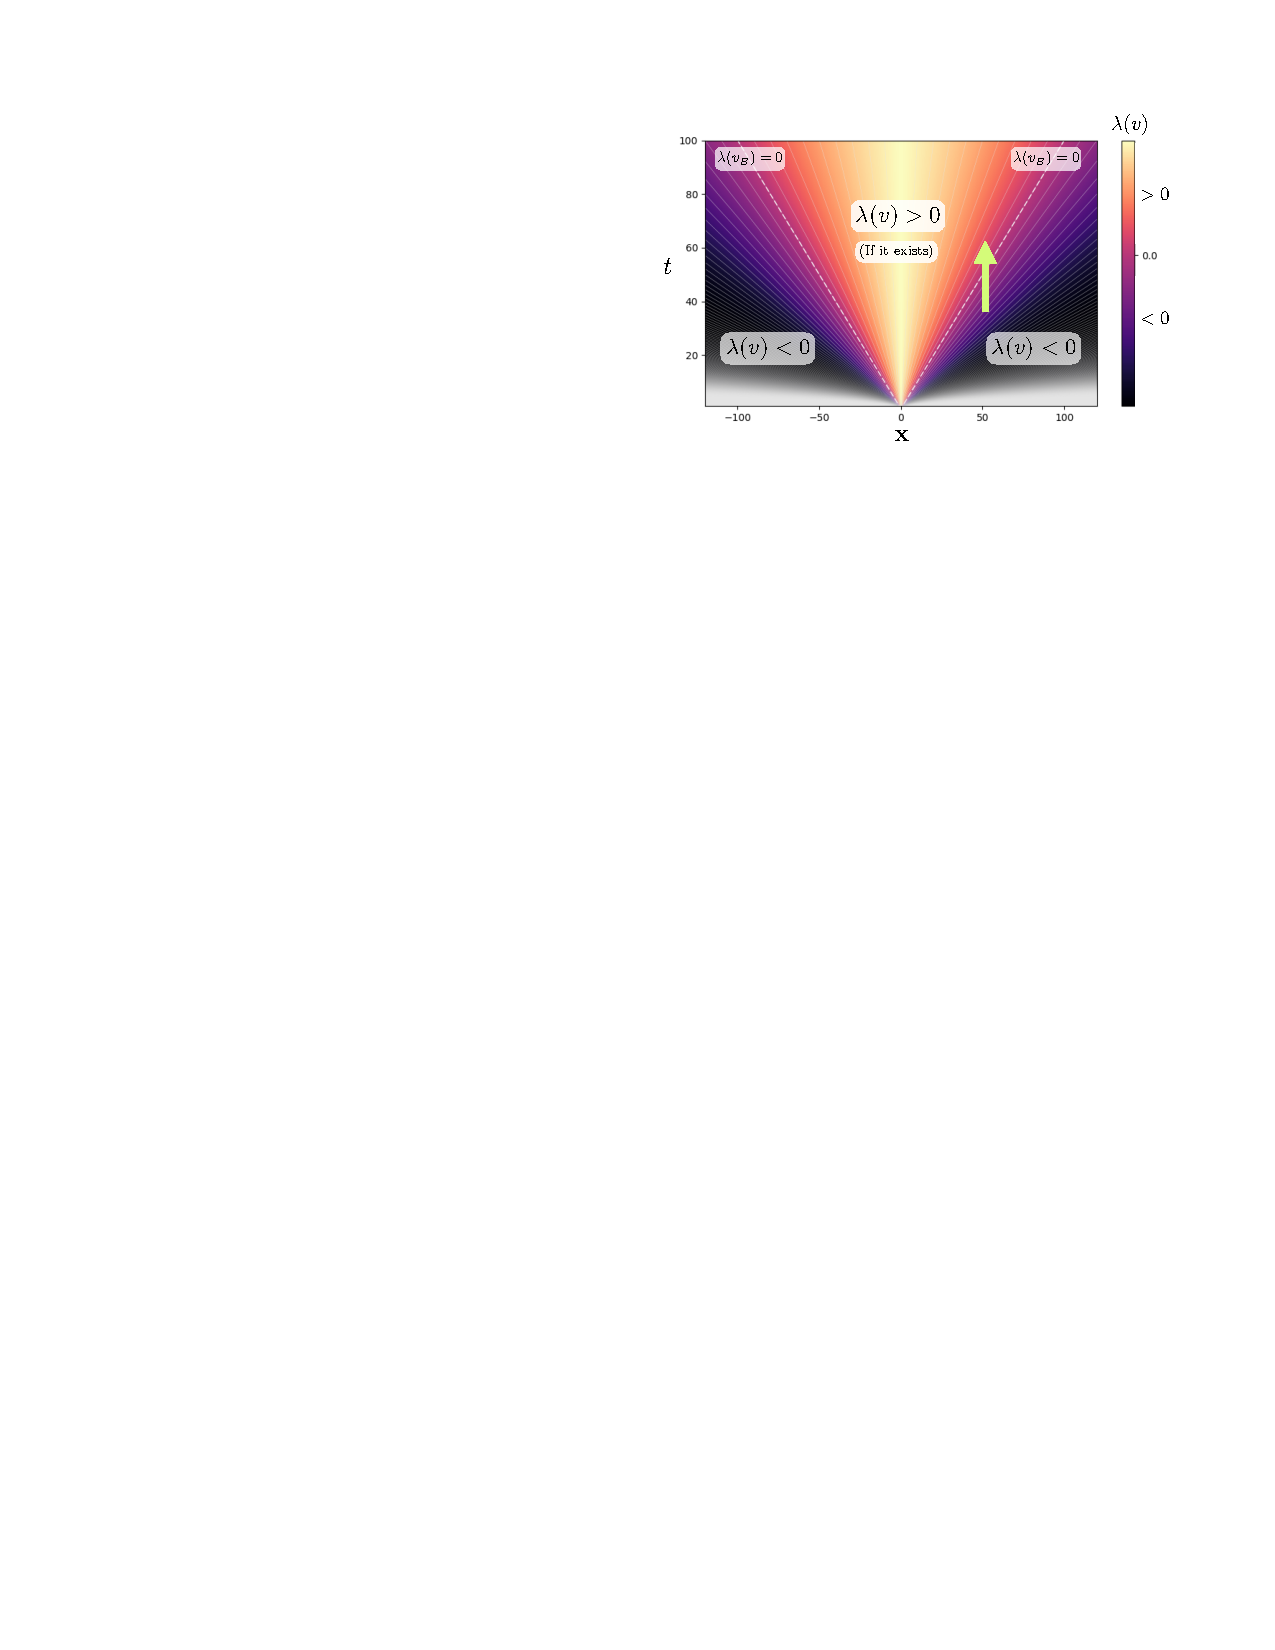
\includegraphics[width=.7\textwidth]{khemani_lambda}
	\caption{Initially local information, spreading [Khemani, Huse, Nahum, 2018].}
\end{figure}
\end{frame}

\begin{frame}{Measures of thermalization}
We want to measure the spreading of ``information"\\
But how can we quantify this information and see how it spread?
\begin{itemize}
	\item Operator right weight, $\rho_R(i,t)$
	\item Out-of-time-order commutator (OTOC), $C(i,t)$
	\item Bipartite entanglement entropy, $S(x,t)$
\end{itemize}
\end{frame}

\begin{frame}{Operator right weight, $\rho_R(i,t)$}
The Pauli matrices ($X,Y,Z,I$) form a basis for single site operators. \\
Pauli strings ($I_1\otimes Z_2\otimes X_3\otimes I_4$, etc.) form a basis for single site operators.\\
How many of these basis operators (weighted) end on site $i$?\\
If we write $\mathcal{O} = \sum c_j \mathcal{O}_j,\; j=1,\dots,q^{2L}$, then
\begin{align}
\rho_R(i,t) = \sum_{\mathcal{O} \text{ ends on $i$}}|c_i|^2. \nonumber       
\end{align}
By unitarity, $\sum_i \rho_R(i,t)=1$.\\
Not a density operator.
\end{frame}

\begin{frame}{Operator right weight, $\rho_R(i,t)$}
Example:
\begin{align}
\mathcal{O} &= \sqrt{\th{5}} IIXZI + \sqrt{\frac{2}{5}} IZXIII + \sqrt{\frac{2}{5}} XIIIZ,\nn
\rho_R(1) &= \rho_R(2) = 0,\nn
\rho_R(3) &= \frac{2}{5},\nn
\rho_R(4) &= \frac{1}{5},\nn
\rho_R(5) &= \frac{2}{5}.\nonumber
\end{align}
In general, these will depend on time.
\end{frame}

\begin{frame}{Out-of-time-order commutator}
Another option, the OTOC:
\begin{align*}
C(i,t) &= \half\ex{|[\mathcal{O}_0(t), W_i]|^2},
\end{align*}
with $\mathcal{O}_0$ initially local, $W_i=I_1\cdots I_{i-1}W_iI_{i+1}\cdots I_L$ and $W=X,Y$, or $Z$ at site $i$.
\end{frame}

\begin{frame}{Connection}
Average the OTOC over choices of $W$. This then measures the weight of non-identity operators at site $i$.\\
OTOC saturates at late time (generically), while right weight has a traveling `pulse.'
\end{frame}

\begin{frame}{Connection}
\begin{columns}
	\begin{column}{0.5\textwidth}  %%<--- here
		\begin{figure}
			\centering
			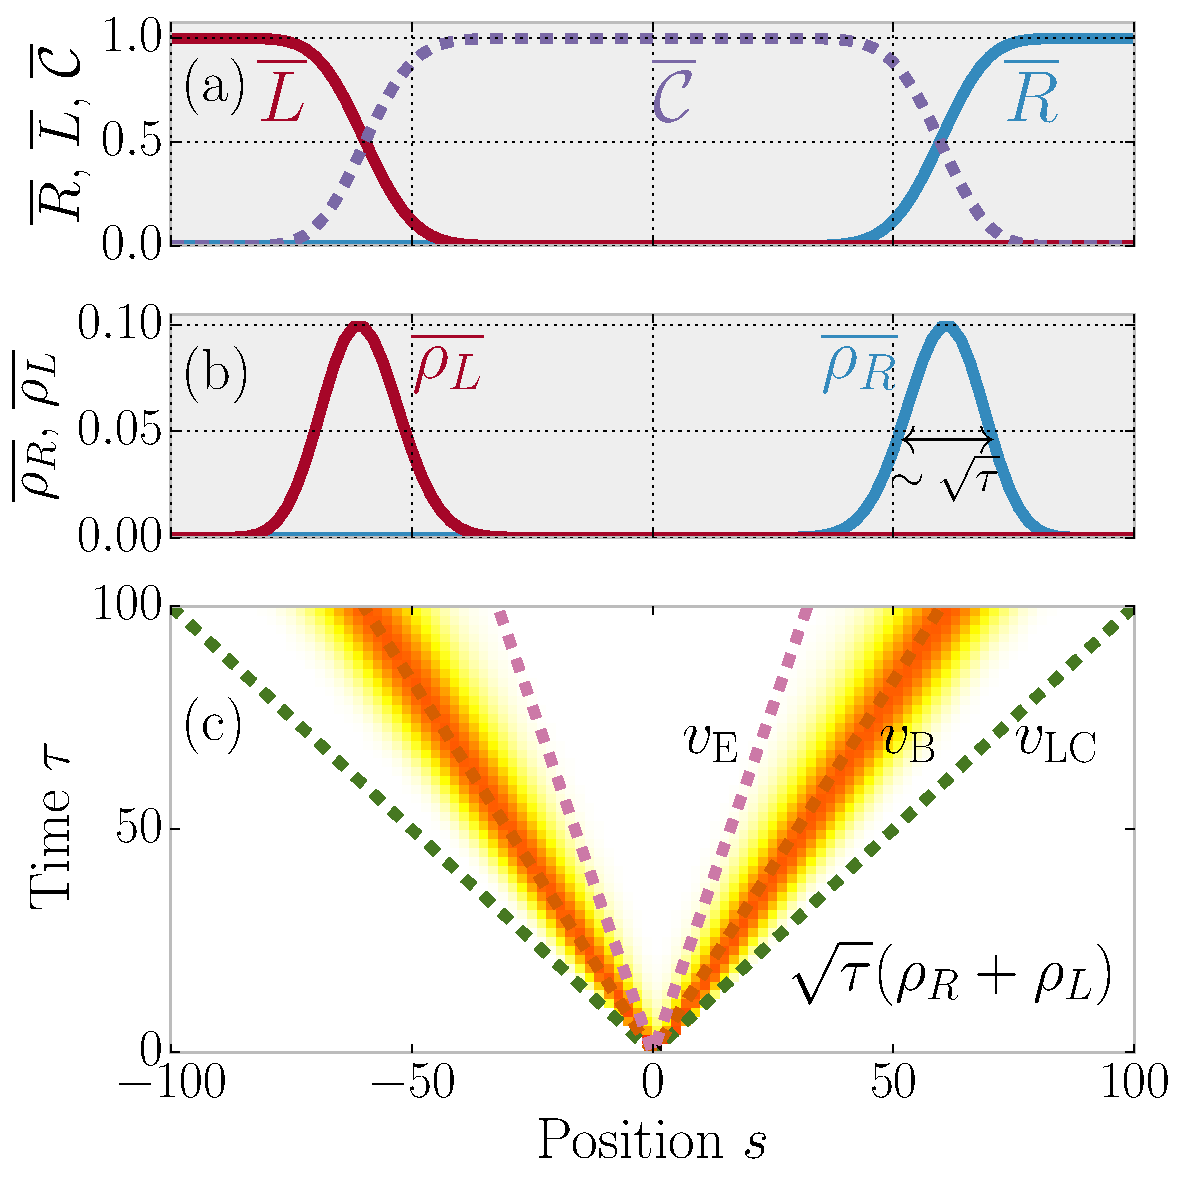
\includegraphics[width=\textwidth]{onesite_spreading}
		\end{figure}
	\end{column}
	\begin{column}{0.5\textwidth}
		Compare the integrated right (and left) weights and the OTOC (properly scaled).\\
		\bigskip
		The right weight is a pulse that diffuses with width $\sim \sqrt{t}$.\\
		\bigskip
		\bigskip
		Right and left weights spreading and diffusing in time [von Keyserlingk, Rakovszky, Pollmann, Sondhi, 2017]
		\bigskip
	\end{column}
\end{columns}
\end{frame}

\section{Time-independent Hamiltonians}

\begin{frame}{Time-independent Hamiltonian}
\begin{itemize}
	\item Sites with finite Hilbert space, dimension $q$
	\item Not relativistic: no limit to information speed
	\item \emph{Most} information still travels at finite speed: Lieb Robinson bounds [Lieb, Robinson, 1972]
	\item OTOC is exponentially small outside ``lightcone"
\end{itemize}
\end{frame}

\begin{frame}{Velocity-dependent Lyapunov exponent}
For a set velocity, $C_W(i = vt, t) \sim e^{\lambda(v)t}$
\begin{figure}
	\centering
	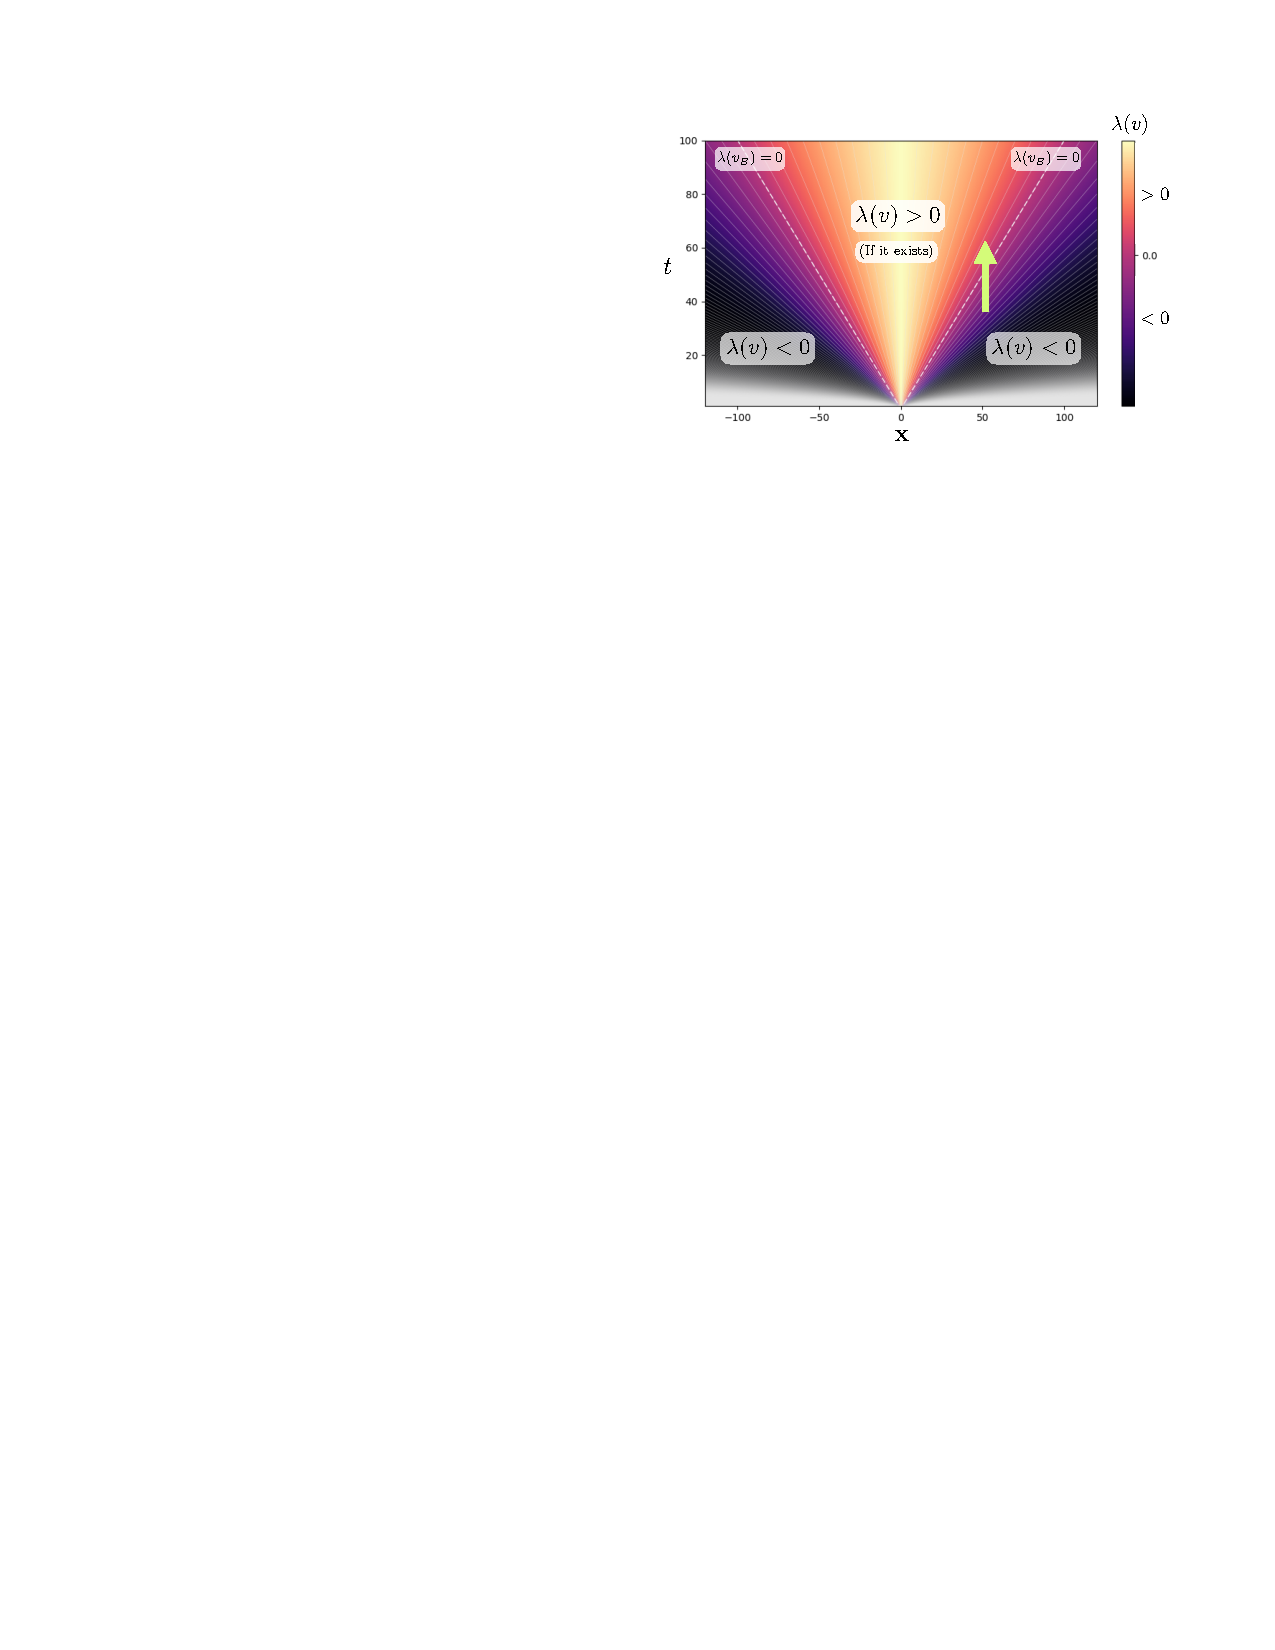
\includegraphics[width=.7\textwidth]{khemani_lambda}
	\caption{Lyapunov exponent at various velocities [Khemani, Huse, Nahum, 2018].}
\end{figure}
\end{frame}

\begin{frame}{Velocity-dependent Lyapunov exponent}
Behavior of VDLEs
\begin{figure}
	\centering
	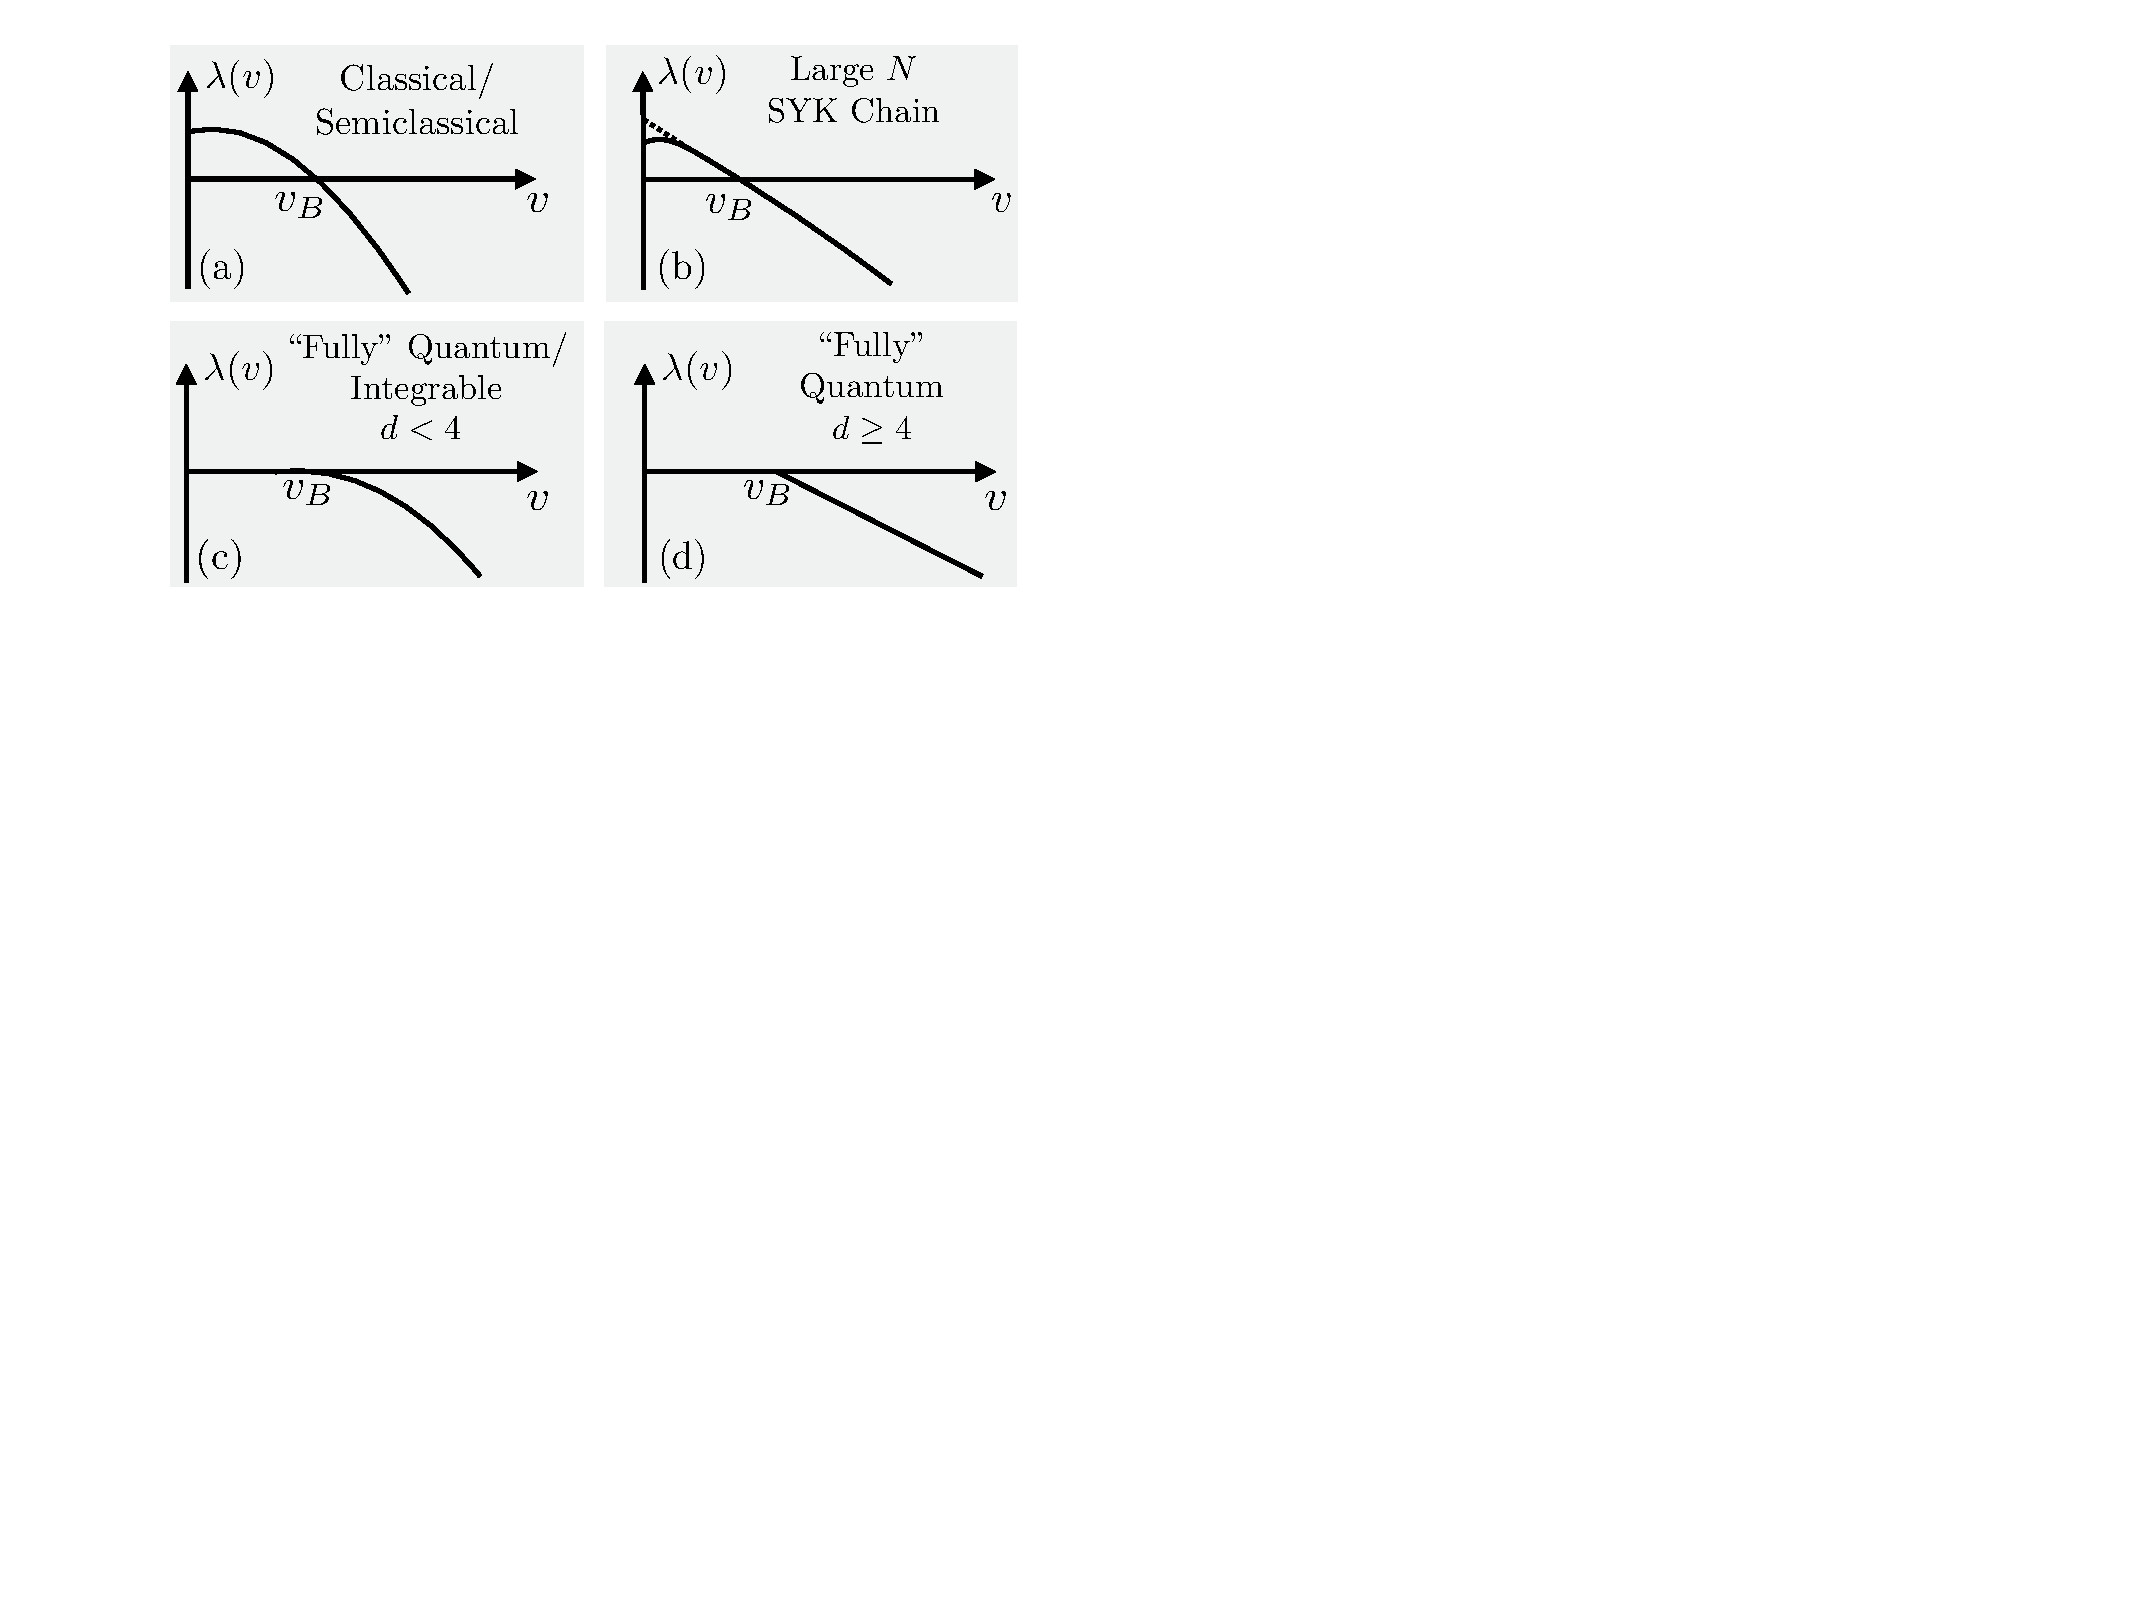
\includegraphics[width=.5\textwidth]{lyapunov}
	\caption{VDLEs for various systems, [Khemani, Huse, Nahum, 2018].}
\end{figure}
$\lambda(v)\sim -(v-v_B)^\alpha$, then $\rho_R$ broadens as $t^\beta$, with  $\beta=\frac{\alpha-1}{\alpha}$.
\end{frame}

\section{Random unitary circuits}

\begin{frame}{Quantum circuits}
\begin{itemize}
	\item Chain of $q$-dimensional sites
	\item Apply unitary operators at discrete times
	\item Information speed is set by circuit architecture
\end{itemize}
\begin{figure}
	\centering
	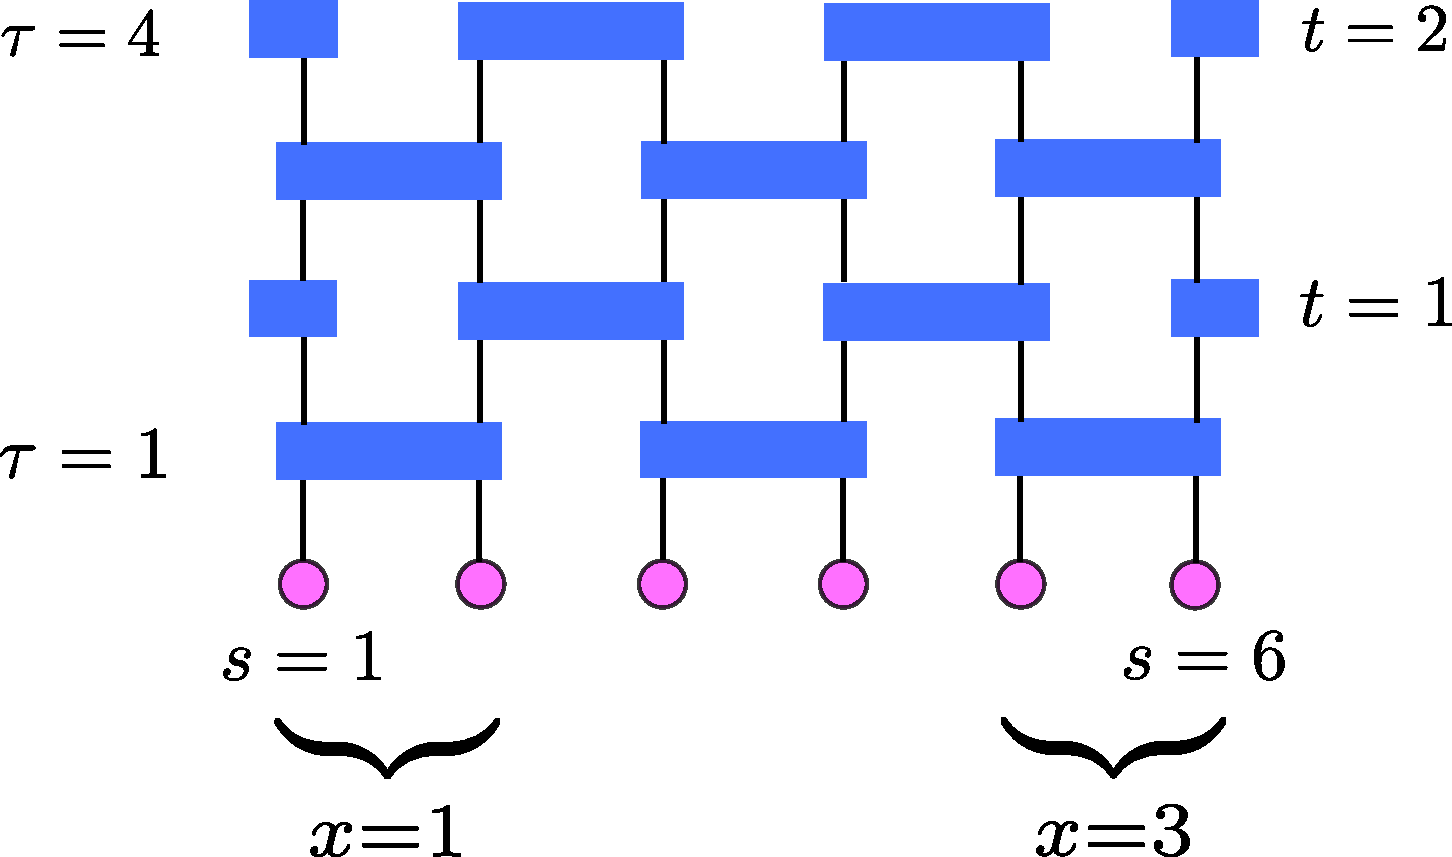
\includegraphics[width=.5\linewidth]{random_circuit}
	\caption{Quantum circuit, [von Keyserlingk, Rakovszky, Pollmann, Sondhi, 2017]}
\end{figure}
\end{frame}

\begin{frame}{Operator hydrodynamics (circuit)}
After one gate [Nahum, Vijay, Haah, 2018],
\begin{align}
\rho(i,\t+1) &= (1-p)\left[\rho(i,\t)+\rho(i+1,\t)\right],\nn
\rho(i+1,\t+1) &= p\left[\rho(i,\t)+\rho(i+1,\t)\right],\nonumber
\end{align}
where $p$ is the probability of moving forwards, 
\begin{align}
p = 1-p_\text{back} = 1-\frac{q^2-1}{q^4-1} = \frac{q^2}{q^2+1}. \nonumber
\end{align}
The problem is that gates don't act everywhere at every time step.
\end{frame}

\begin{frame}{Operator hydrodynamics (circuit)}
After two applications (and some new variables),
\begin{align}
\rho(x,t+1)&=p^2\rho(x-1,t)+2p(1-p)\rho(x,t)+(1-p)^2\rho(x+1,t).\nonumber
%\partial_t\rho(x,t) &= v_B(q)\partial_x\rho(x,t) + D(q)\partial_x^2 \rho(x,t). \nonumber
\end{align}
This is a biased random walk with
\begin{align}
v_B(q) = p^2 - (1-p)^2 = \frac{q^2 +1}{q^2-1},\quad D(q)=\frac{q/2}{q^2 +1},\nonumber
\end{align}
where
\begin{align}
\ex{x} -  x_0 = v_Bt,\quad \ex{x^2} - \ex{x}^2 = 2Dt.\nonumber
\end{align}
Exact limit as $q\to\infty$.
\end{frame}

\begin{frame}{Recall}
\begin{figure}
	\centering
	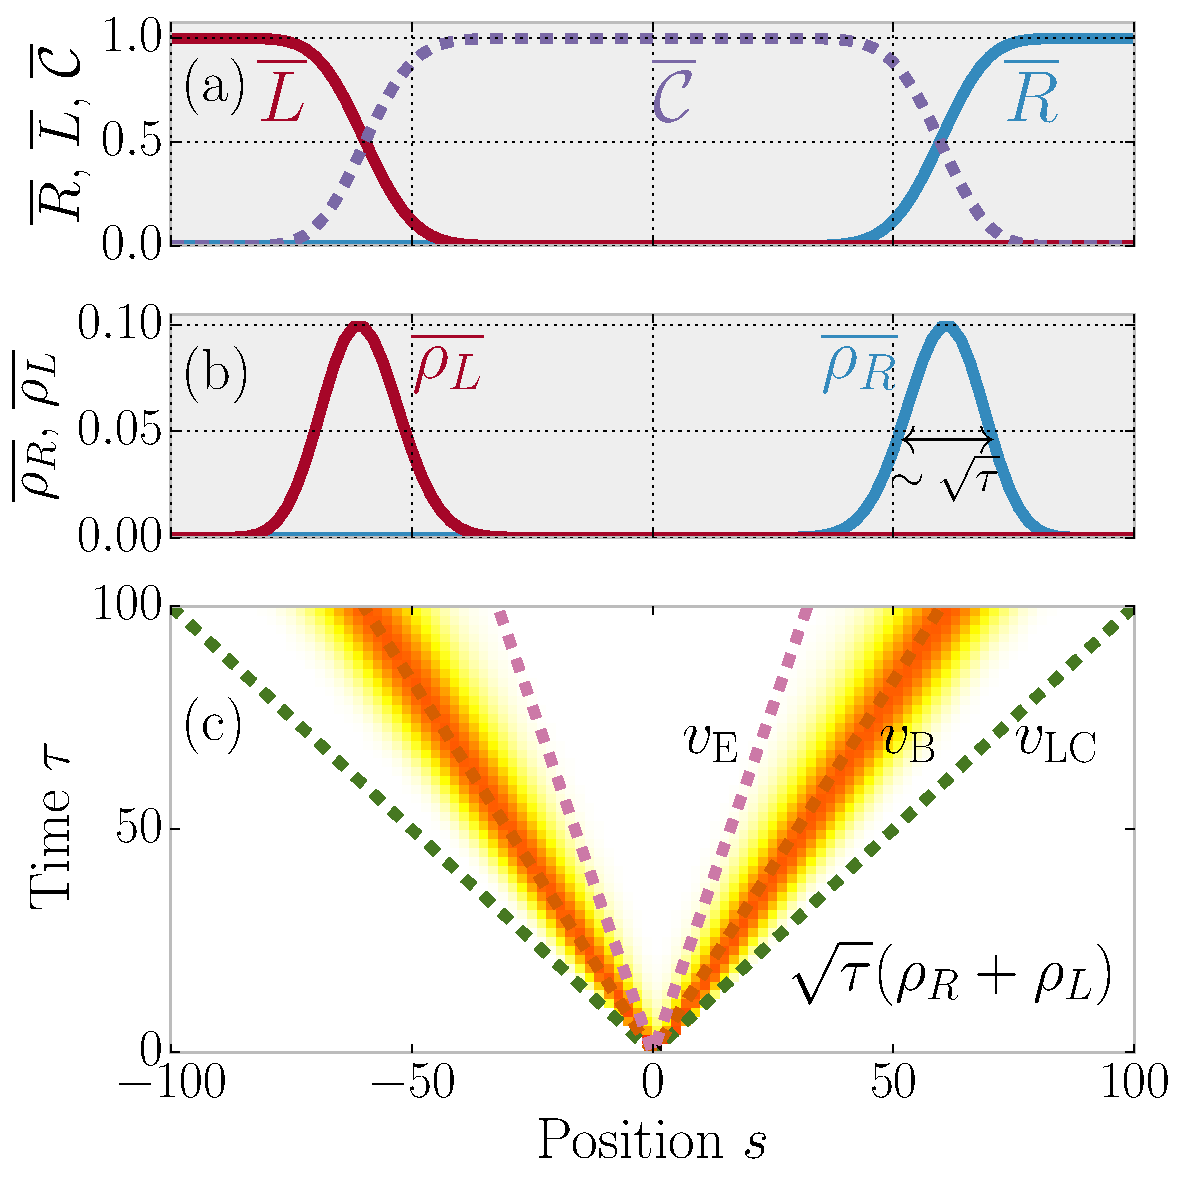
\includegraphics[width=.5\textwidth]{onesite_spreading}
\end{figure}
\end{frame}

\begin{frame}{Operator hydrodynamics (Hamiltonian)}
Floquet system: ``kicked Ising model"
\begin{align}
U = e^{-i \frac{T}{2} h \sum_s X_s} e^{-i\frac{T}{2}\sum_s[Z_sZ_{s+1} + gZ_s]}. \nonumber
\end{align}
\begin{columns}
	\begin{column}{0.4\textwidth}  %%<--- here
		\begin{figure}
			\centering
			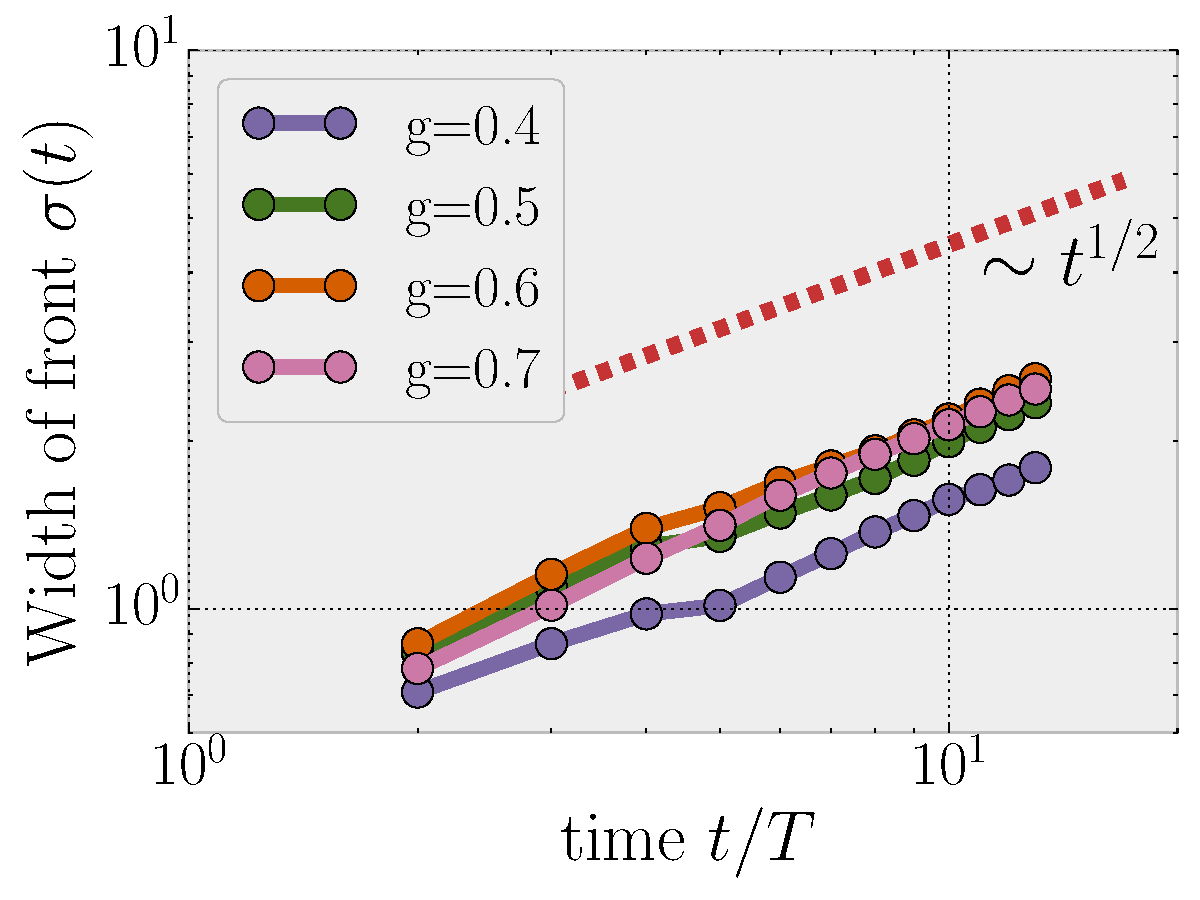
\includegraphics[width=\textwidth]{kicked_width}
		\end{figure}
	\end{column}
	\begin{column}{0.7\textwidth}
		Diffusive broadening of operator front exists at various values of $g$ [von Keyserlingk, Rakovszky, Pollmann, Sondhi, 2017].
	\end{column}
\end{columns}
\end{frame}

\section{Conclusion}

\begin{frame}{More cool stuff}
Wait a minute! That wasn't a time independent Hamiltonian!
\begin{itemize}
	\item Conserved quantities
	\item Any Hamiltonian conserves energy
	\item Leads to more complicated (slower) dynamics
	\item But you can still model this with circuits!
	\item With enough conserved quantities, the circuit can localize [Pai, Pretko, Nandkishore, 2019]
\end{itemize}
\end{frame}

\begin{frame}
Summary
\begin{itemize}
	\item Concept of thermalization
	\item Measures of thermalization
	\item Thermalization in circuits
	\item thermalizations in Hamiltonians (kinda\dots)
\end{itemize}
\end{frame}

\begin{frame}{Alternative: localization*}
Maybe some information doesn't spread out.\\
\begin{itemize}
	\item Quantum phase transition [Pal, Huse, 2010]
\end{itemize}
\begin{align}
H=􏰜\sum_{i=1}^{L}[h_iS_i^z+J\vec{S}_i\cdot\vec{S}_i]\nonumber
\end{align}
\begin{figure}
	\centering
	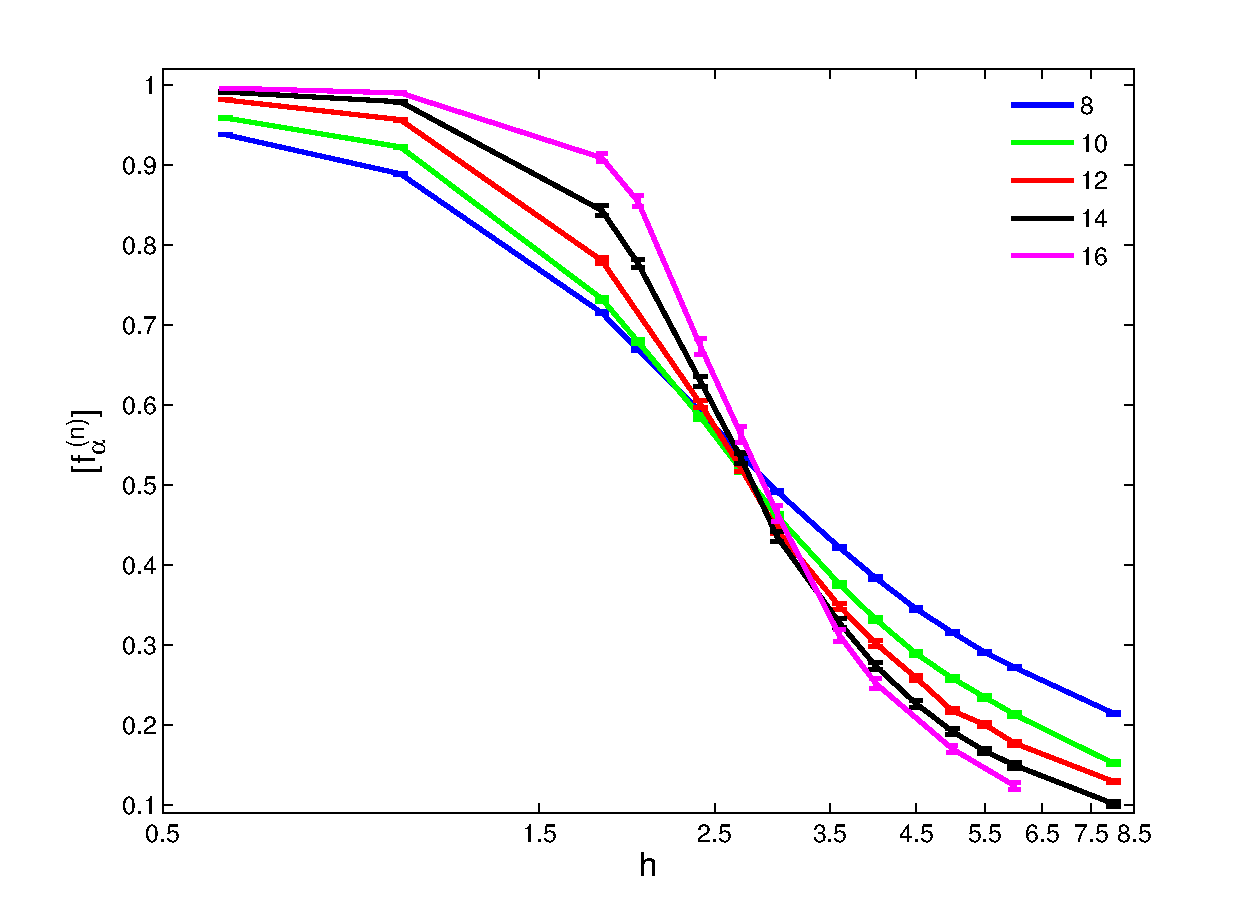
\includegraphics[width=.45\linewidth]{spin_mobility}
	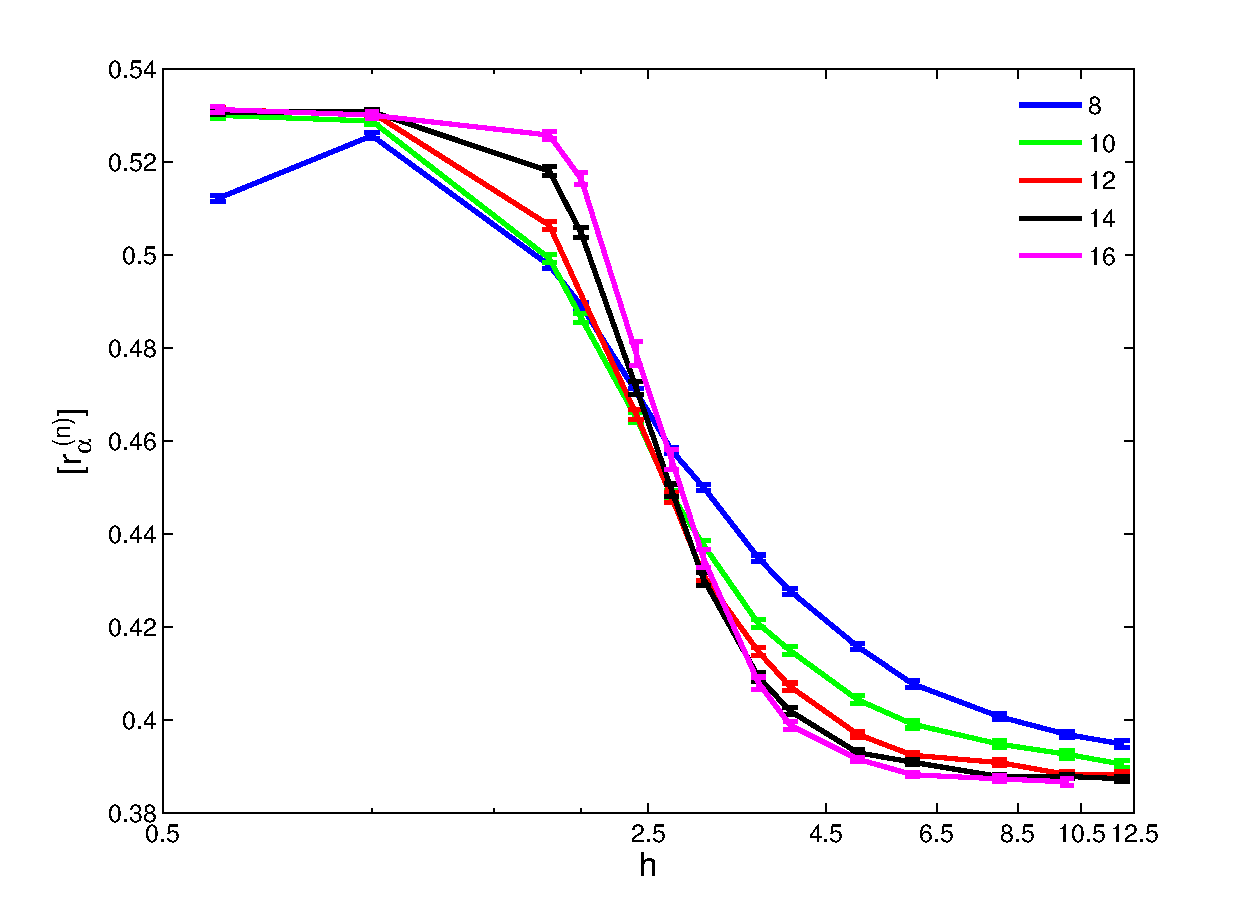
\includegraphics[width=.45\linewidth]{energy_gaps}
	\caption{Spin mobility (L) and relative gaps between energy eigenvalues (R)}
\end{figure}
\end{frame}

\begin{frame}{Bipartite entanglement entropy*}
Another useful measure of information spreading, this time spreading of entanglement (Fig. from [Nahum, Ruhman, Vijay, Haah, 2016])
\begin{figure}
	\centering
	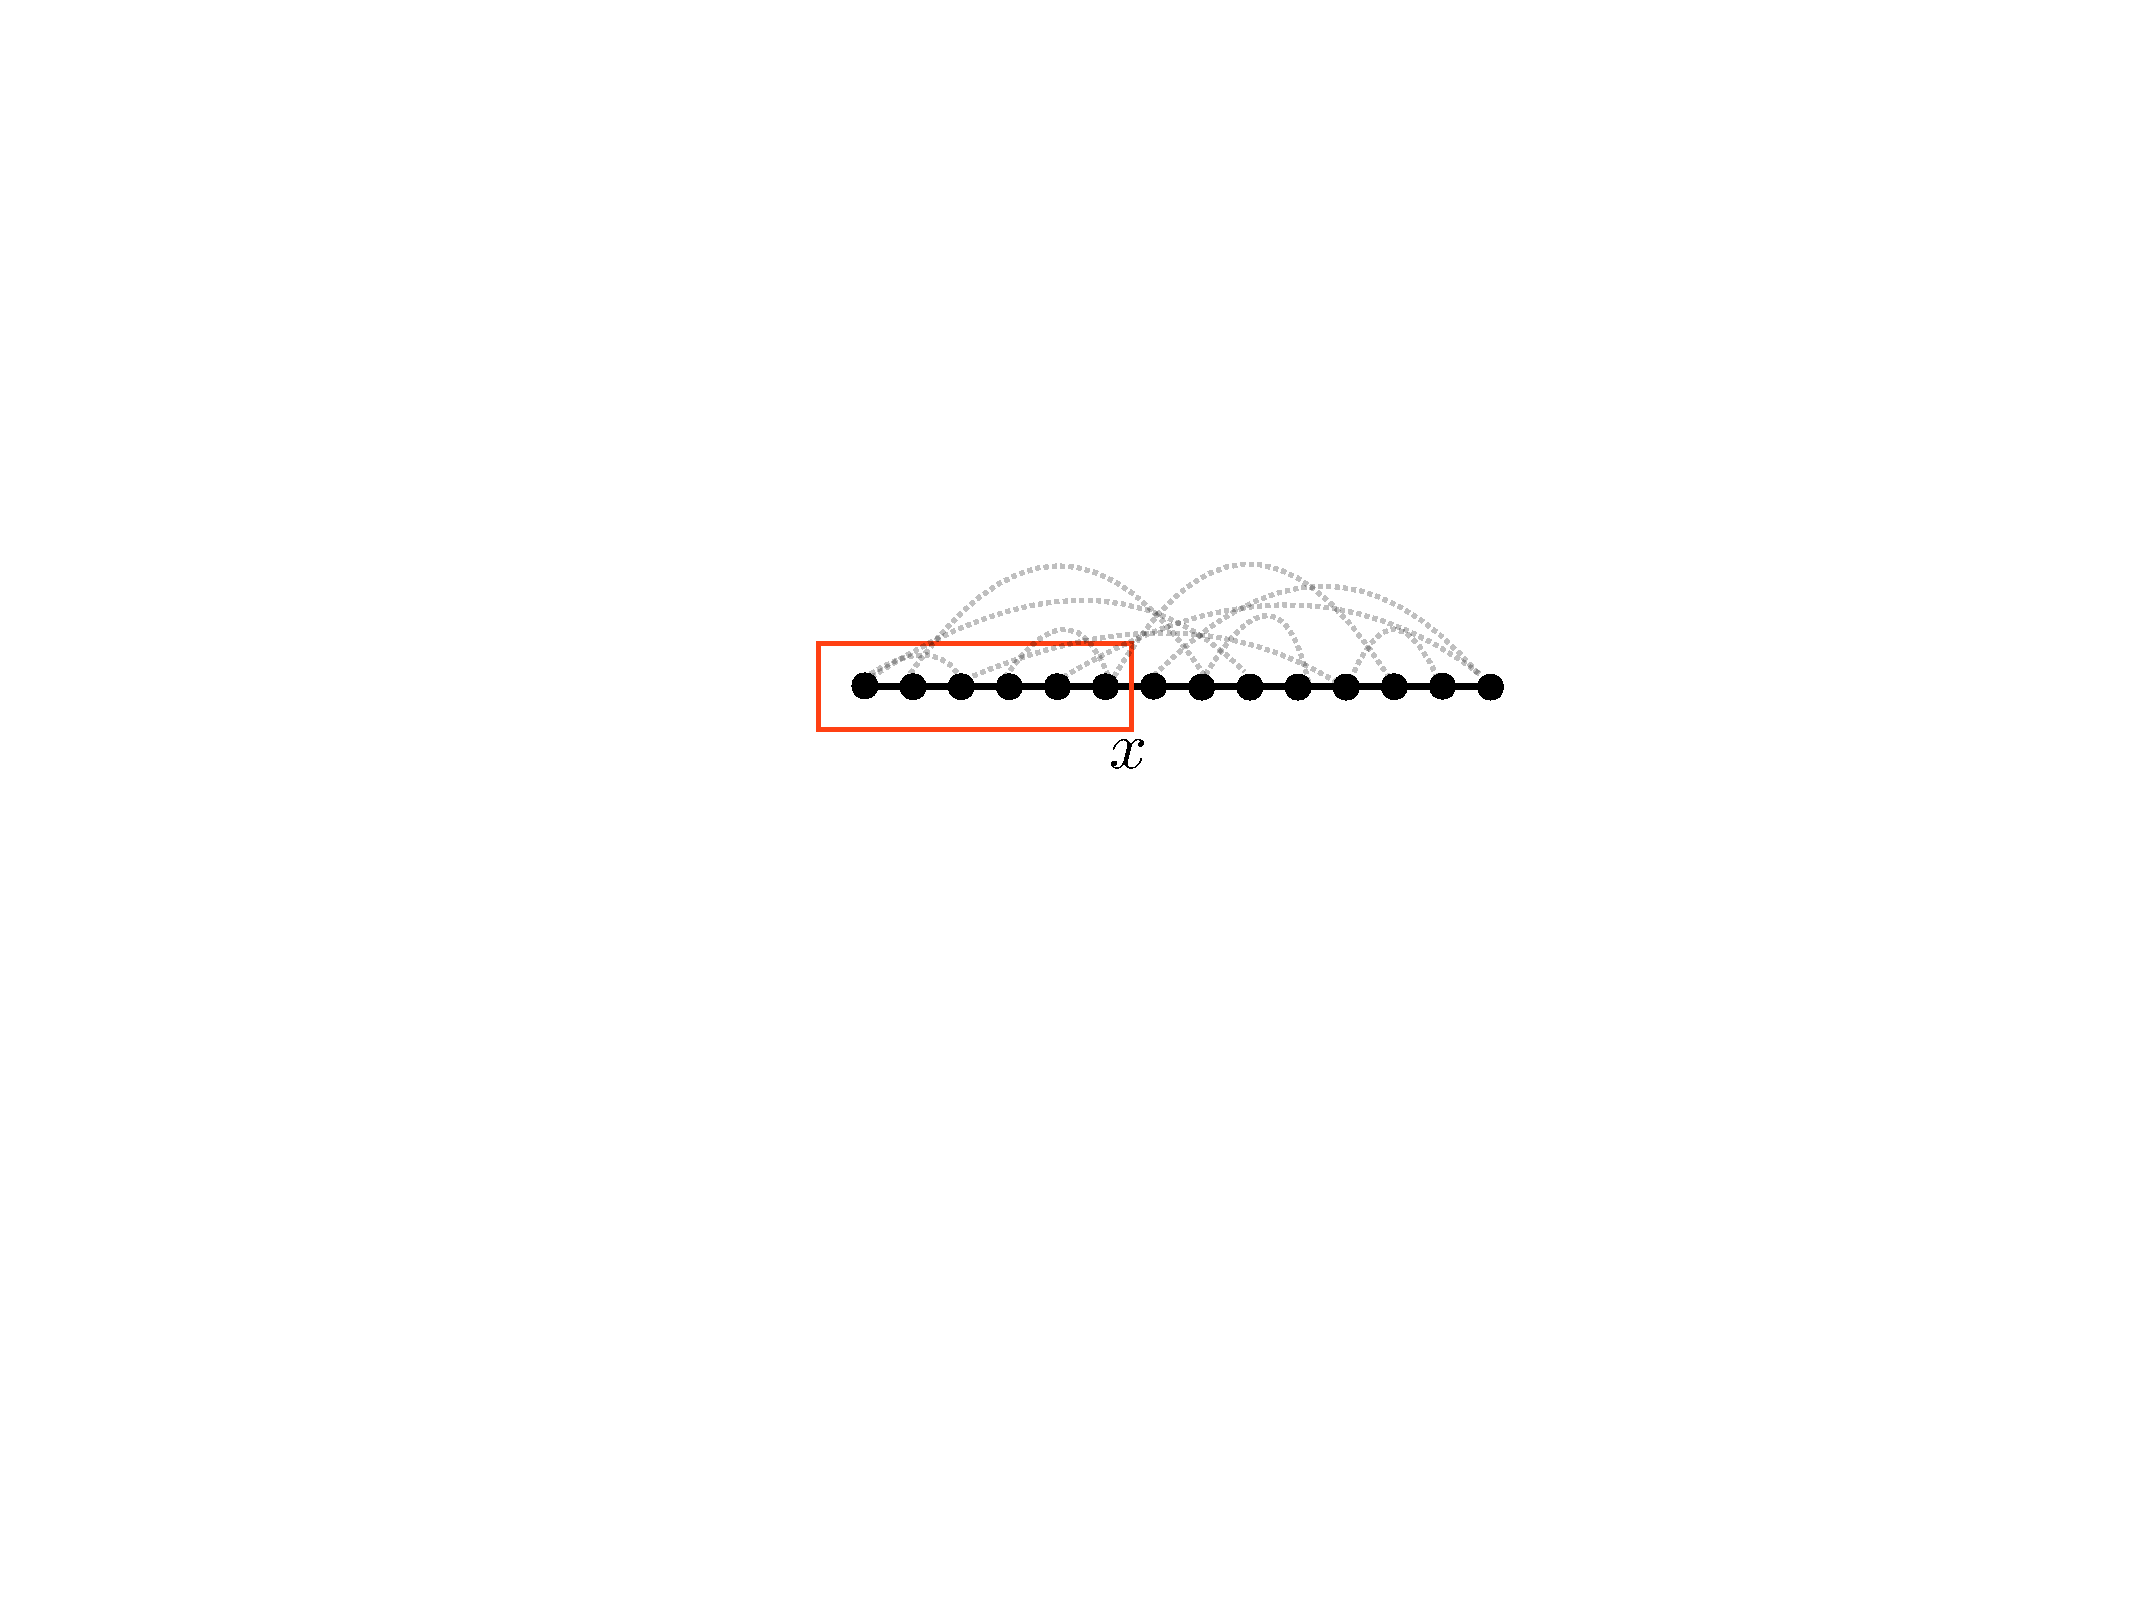
\includegraphics[width=.6\textwidth]{spinchainfig}
\end{figure}
Entropy across a cut at bond $x$.
\begin{align}
S(x,t) = -\Tr \rho_x\log\rho_x,\nonumber
\end{align}
where $\rho_x$ is the reduced density matrix on one side of $x$,
\begin{align}
\rho_x=\Tr\limits_{\text{left}}\rho.\nonumber
\end{align}
\end{frame}

\end{document} 